\section{Sensor calibrations}

\subsubsection{Camera}
To find the transformation from the camera frame to the body frame, both the intrinsic parameters and the extrinsic parameters of the camera had to be found. The intrinsic parameters where found using Kalibr\cite{Kalibr1}\cite{Kalibr2}\cite{Kalibr3}, by filming an april grid (figure \ref{Fig:Aprilgrid}) at various angles and distances, and running the whole film through Kalibr. This gives the distortion of the camera with respect to the world, such that using this transformation it was possible to find all the points in the world corresponding to a single pixel in the image frame. 

The extrinsic parameters, i.e. the transformation from the camera to the CG, where found by simply measuring by hand the translation and rotation from the camera to the body-frame. Attempts where made at using the Kalibr tool for this too, by having it find the transformation between camera and IMU. This worked well on our test trolley, as the test trolley was light enough for us to lift around, giving it the necessary pitch, roll and yaw for the algorithm to work. The car was however not light enough for this, so hand-measurements will have to suffice.

\begin{figure}
    \centering
    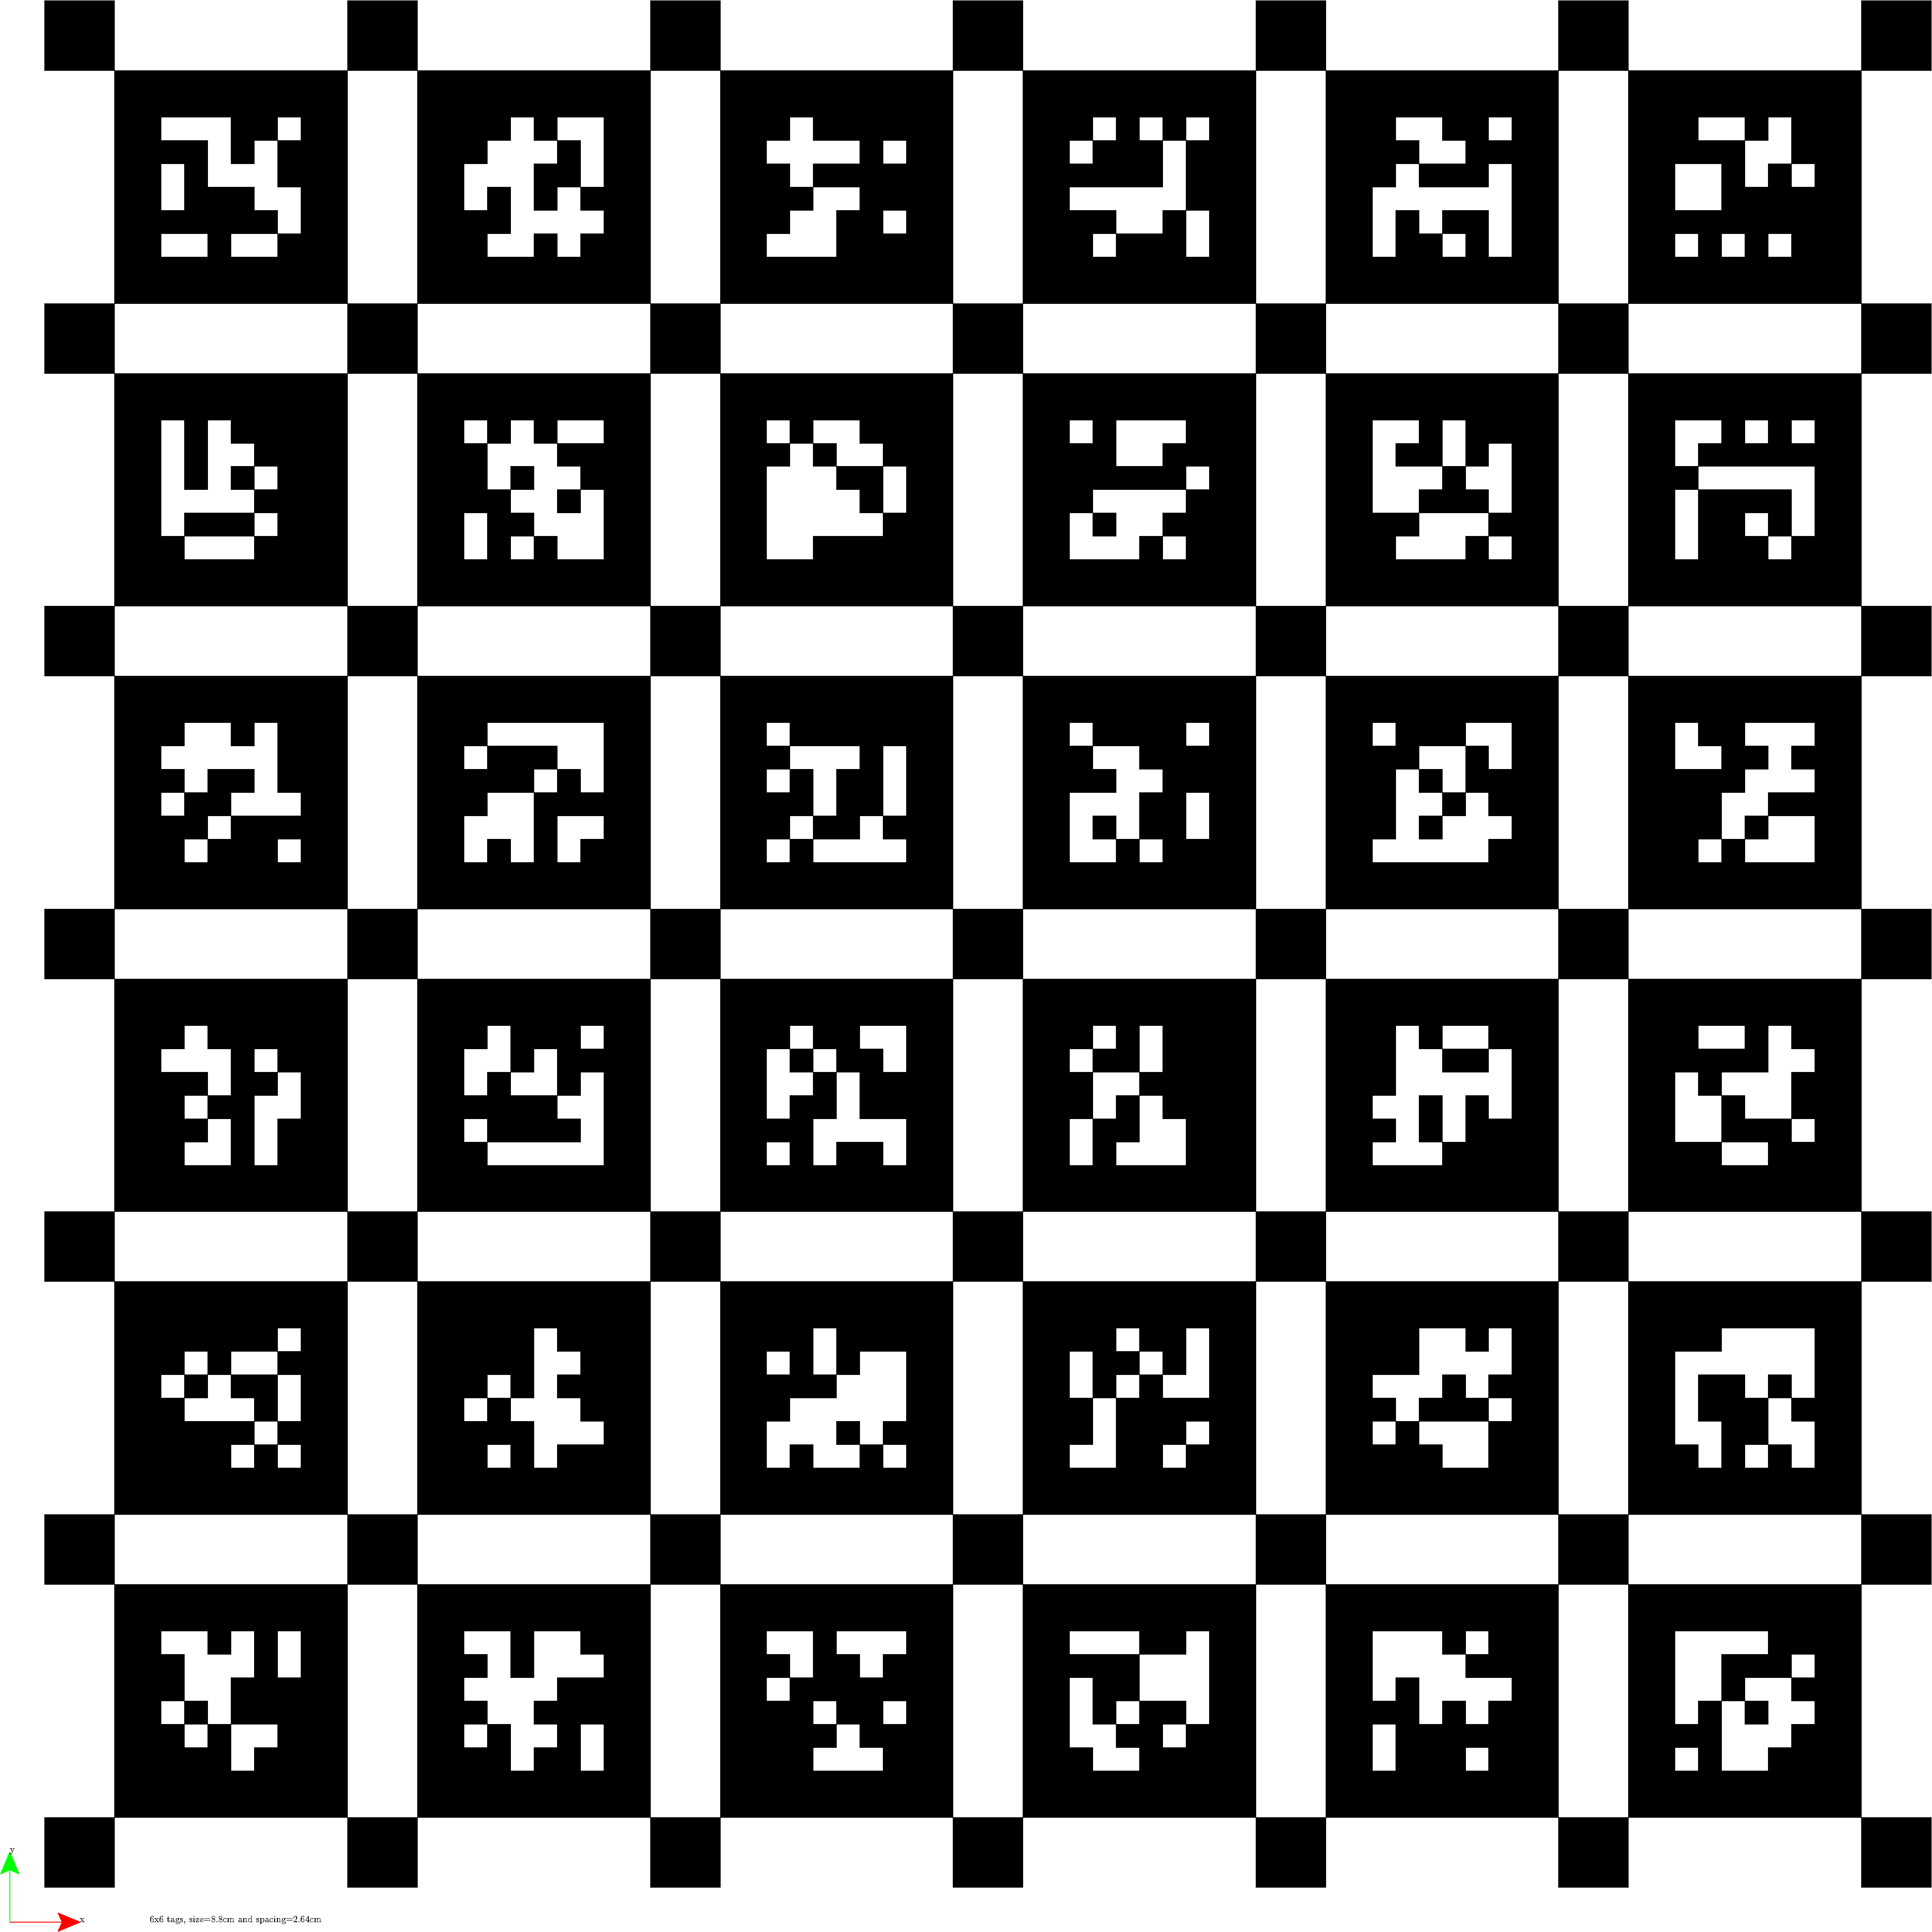
\includegraphics[width=0.5\linewidth]{0_Images/4_Implementation/aprilgrid.pdf}
    \caption[Aprilgrid, the grid used for camera calibration.]
    {Aprilgrid, the grid used for camera calibration.}
    \label{Fig:AprilGrid}
\end{figure}

\subsubsection{IMU}

Even though the IMU came with a factory calibration, it was a general one supposed to cover all Vectornav VN300s. So, in order to get a better measurement covariance matrix to send to the built in Kalman filter in the IMU, steps were taken to find the covariance of this specific device. This was done by again using the Kalibr toolbox, but this time for IMU calibration. The device was left alone on a vibration free desk for 8 hours, while recording its output. The output was sent through Kalibr, and the new estimate of the covariance matrix was outputted. This was in turn set to the default value of the VN300. 

Finding the transformation from the IMU to the body frame was easy as the IMU was placed at what CAD-models in SolidWorks said was the CG. This was done so some of the math in the state estimation algorithm would become easier.

\subsubsection{LiDARS}

To find the transformation from the two LiDARs to the body frame, the transformation from one of them to CG was found by hand measurements. The other one was found by having both LiDARs see a thin stick held stationary. One of the LiDARs where then transformed by trial and error until they both output the same value for the location of the stick. 